\chapter{Microservices}
\label{bab:mikroservis}

\section*{Tujuan Pembelajaran}

\begin{enumerate}
  \item Menjelaskan aturan satu layanan satu basis data beserta akibatnya bagi
    penyusunan laporan yang membutuhkan data beberapa layanan.
  \item Membedakan mikroservis dari \textit{service-based architecture}, lalu
    menentukan kapan pembagian sehalus ini layak dipilih.
  \item Mengukur latensi beserta jumlah lompatan permintaan gabungan, harga
    penggabungan di dalam kode, dan jumlah permintaan yang gagal selama satu
    layanan dirilis ulang.
\end{enumerate}

\section{Pendahuluan}

Mikroservis membagi sebuah sistem menjadi banyak layanan kecil yang masing-masing
berjalan di prosesnya sendiri. Setiap layanan mengurus satu kemampuan bisnis,
menyimpan datanya sendiri, lalu dirilis tanpa menunggu layanan lain. Lewis dan
Fowler mencatat sejumlah ciri gaya ini, dan salah satu yang paling menentukan
adalah pengelolaan data yang tidak lagi dipusatkan~\cite{lewis2014microservices}.

Ciri itulah yang membedakan bab ini dari Bab~11. Di sana layanan memang sudah
dipisah menjadi beberapa proses, namun seluruhnya masih membaca satu basis data
yang dipakai bersama. Di sini basis datanya ikut dipecah, sehingga satu layanan
tidak pernah membaca tabel milik layanan lain. Perbedaan yang terdengar kecil
itu mengubah hampir segalanya, mulai dari cara menyusun laporan sampai cara
memasang perbaikan.

Bab ini membandingkan dua versi dari satu domain yang sama, yaitu pemesanan
penukaran valuta asing di sebuah bank. Versi pertama berupa monolit dengan satu
basis data, sedangkan versi kedua berupa tiga layanan dengan tiga basis data
ditambah satu gerbang. Pembahasannya mengikuti kerangka Richards dan
Ford~\cite{richards2020fundamentals} serta catatan Newman tentang kepemilikan
data pada setiap layanan~\cite{newman2021building}.

\section{Satu Layanan, Satu Basis Data}

Aturannya hanya satu kalimat. Sebuah layanan memegang basis datanya sendiri, dan
layanan lain tidak boleh membuka basis data itu, bahkan untuk sekadar membaca.
Newman menyebut kemandirian rilis sebagai sifat terpenting mikroservis, dan
sifat itu gugur begitu dua layanan berbagi satu tabel~\cite{newman2021building}.
Sebab, tabel yang dipakai bersama berubah menjadi antarmuka bersama yang tidak
pernah disepakati.

Aturan tersebut punya dua konsekuensi praktis. Pertama, tidak ada satu kueri
Structured Query Language (SQL) pun yang boleh menyentuh dua basis data
sekaligus, sehingga penggabungan data pindah dari mesin basis data ke kode
pemanggilnya. Kedua, matinya satu layanan tidak lagi otomatis mematikan yang
lain, sebab tidak ada sumber daya bersama yang ikut hilang.

Gambar~\ref{fig:batas-data} memperlihatkan batas tersebut pada contoh bab ini.
Garis putus-putus hijau adalah batas layanan sekaligus batas datanya, sedangkan
panah merah adalah jalur yang dilarang.

\begin{figure}[htbp]
  \centering
  \begin{tikzpicture}[
    layanan/.style={draw, rounded corners=2pt, minimum width=2.5cm,
      minimum height=0.7cm, align=center, font=\scriptsize\bfseries},
    simpan/.style={draw, cylinder, shape border rotate=90, aspect=0.25,
      minimum height=0.6cm, minimum width=1.5cm, align=center,
      font=\tiny\bfseries},
    panah/.style={-{Stealth[length=2mm]}, thick},
    larangan/.style={-{Stealth[length=2mm]}, thick, dashed, red!70},
    batas/.style={draw, dashed, rounded corners=4pt, praditagreen,
      inner sep=5pt}
  ]
    \node[layanan, fill=blue!8] (nasabah) at (0,0) {nasabah};
    \node[layanan, fill=blue!8] (pesanan) at (3.2,0) {pesanan};
    \node[layanan, fill=blue!8] (kurs) at (6.4,0) {kurs};

    \node[simpan, fill=green!10, below=0.75cm of nasabah] (dbn) {nasabah.db};
    \node[simpan, fill=green!10, below=0.75cm of pesanan] (dbp) {pesanan.db};
    \node[simpan, fill=green!10, below=0.75cm of kurs] (dbk) {kurs.db};

    \draw[panah] (nasabah) -- (dbn);
    \draw[panah] (pesanan) -- (dbp);
    \draw[panah] (kurs) -- (dbk);

    \node[batas, fit=(nasabah)(dbn)] (bn) {};
    \node[batas, fit=(pesanan)(dbp)] (bp) {};
    \node[batas, fit=(kurs)(dbk)] (bk) {};

    \node[layanan, fill=praditagreen!25, minimum width=3.4cm] (gerbang)
      at (3.2,2.1) {Gerbang\\{\tiny\mdseries tanpa basis data}};

    \draw[panah] (gerbang) -- (nasabah);
    \draw[panah] (gerbang) -- (pesanan);
    \draw[panah] (gerbang) -- (kurs);

    \draw[larangan] (pesanan.west) to[out=200, in=20]
      node[font=\tiny, above left=-1pt and -4pt] {dilarang} (dbn.east);
  \end{tikzpicture}
  \caption{Batas layanan berimpit dengan batas datanya. Gerbang tidak memegang
    basis data, sehingga seluruh datanya diminta lewat jaringan}
  \label{fig:batas-data}
\end{figure}

Analoginya ada di kampus. Bayangkan tiga loket yang berdiri sendiri, yaitu
loket kemahasiswaan, loket keuangan, dan loket perpustakaan. Masing-masing
memegang buku catatannya sendiri, dan petugas satu loket tidak pernah
membuka buku loket sebelah. Surat keterangan bebas tanggungan karena itu
menuntut kunjungan ke ketiga loket, lalu isinya disalin menjadi satu lembar.
Kerepotan itu ada harganya, namun ada imbalannya juga, sebab loket perpustakaan
yang tutup tidak menghentikan pelayanan dua loket lain.

Perbedaan dengan Bab~11 terletak pada satu baris saja, dan
Tabel~\ref{tab:sba-mikro} merangkumnya.

\begin{table}[htbp]
  \centering
  \caption{\textit{Service-based architecture} pada Bab~11 dibanding mikroservis
    pada bab ini}
  \label{tab:sba-mikro}
  \begin{tabularx}{\textwidth}{|l|X|X|}
    \hline
    \textbf{Yang dibandingkan} & \textbf{\textit{Service-based}} & \textbf{Mikroservis} \\
    \hline
    Basis data & Satu, dipakai bersama seluruh layanan & Satu per layanan, tidak dipakai bersama \\
    \hline
    Penggabungan data & Satu kueri SQL dengan JOIN & Beberapa panggilan lalu digabung di dalam kode \\
    \hline
    Rilis satu layanan & Mungkin, selama skemanya tidak berubah & Mungkin, termasuk ketika skemanya berubah \\
    \hline
    Matinya satu layanan & Layanan lain tetap jalan, kecuali basis datanya ikut mati & Layanan lain tetap jalan, dan basis datanya terpisah \\
    \hline
    Ukuran layanan & Kasar, beberapa kemampuan besar & Halus, satu kemampuan per layanan \\
    \hline
  \end{tabularx}
\end{table}

Pemisahan itu tampak langsung pada berkas basis datanya.
Listing~\ref{lst:siapkan-data} memperlihatkan keluaran skrip penyiapan, dan
kolom terakhirnya menunjukkan jumlah tabel pada tiap berkas.

\begin{lstlisting}[language=bash, caption={Menyiapkan keempat berkas basis data,
  tersedia di \berkas{sources/chapter13/basis_data.py}}, label=lst:siapkan-data]
cd sources/chapter13
python basis_data.py
# Keluarannya:
# layanan_nasabah  data/nasabah.db   1 tabel, 3 baris
# layanan_pesanan  data/pesanan.db   1 tabel, 6 baris
# layanan_kurs     data/kurs.db      1 tabel, 3 baris
# monolit          data/monolit.db   3 tabel, 12 baris
\end{lstlisting}

Isi kedua versi sengaja dibuat sama persis. Monolit memakai objek
\texttt{Tabel} yang sama dengan ketiga layanan, sehingga datanya tidak mungkin
berbeda. Yang berbeda hanya jumlah berkasnya, yaitu tiga berkas berisi satu
tabel melawan satu berkas berisi tiga tabel.

\section{Gerbang yang Menggabungkan di Dalam Kode}

Konsekuensi pertama itulah yang segera terasa. Pertanyaannya, bagaimana sebuah
laporan yang membutuhkan nama nasabah, daftar pesanannya, dan kurs setiap mata
uang disusun bila tidak ada satu kueri pun yang boleh menyentuh ketiganya.

Pada versi monolit pertanyaan itu tidak pernah muncul. Ketiga tabelnya berada
di satu berkas, sehingga mesin basis data mengerjakan penggabungannya sendiri.
Listing~\ref{lst:kueri-laporan} memperlihatkan kuerinya, dan seluruh laporan
selesai dalam satu perjalanan ke basis data.

\begin{lstlisting}[style=SqlStyle, caption={Penggabungan lewat SQL pada versi
  monolit, tersedia di \berkas{sources/chapter13/monolit.py}},
  label=lst:kueri-laporan]
SELECT n.nama, n.kota, n.rekening,
       p.id, p.mata_uang, p.nominal, k.dasar, k.margin
FROM nasabah AS n
JOIN pesanan AS p ON p.id_nasabah = n.id
JOIN kurs AS k ON k.mata_uang = p.mata_uang
WHERE n.id = ? AND p.status = ?
ORDER BY p.id
\end{lstlisting}

Pada versi mikroservis kueri tersebut tidak dapat ditulis sama sekali, sebab
tabel \texttt{nasabah}, \texttt{pesanan}, dan \texttt{kurs} berada di tiga
berkas yang berbeda. Gerbanglah yang menggantikan pekerjaan klausa
\texttt{JOIN}, dan caranya diperlihatkan Listing~\ref{lst:susun-laporan}.

\begin{lstlisting}[style=PythonStyle, caption={Penggabungan di dalam kode pada
  versi mikroservis, tersedia di \berkas{sources/chapter13/gerbang.py}},
  label=lst:susun-laporan]
nasabah = ambil_json(f"{alamat.NASABAH}/nasabah/{id_nasabah}", token)
if nasabah is None:
  return {"galat": "layanan nasabah tidak menjawab"}, 503
jawaban_pesanan = ambil_json(f"{alamat.PESANAN}/pesanan?nasabah={id_nasabah}")
if jawaban_pesanan is None:
  return {"galat": "layanan pesanan tidak menjawab"}, 503
daftar_pesanan = jawaban_pesanan["pesanan"]
kurs = kumpulkan_kurs(daftar_pesanan)
isi = [gabungkan_baris(satu, kurs[satu["mata_uang"]]) for satu in daftar_pesanan]
\end{lstlisting}

Dua baris terakhir itulah inti persoalannya. Pencocokan mata uang dengan kursnya
dikerjakan kode Python atas dua dokumen JavaScript Object Notation (JSON) yang
datang dari dua proses berbeda. Mesin basis data tidak lagi membantu, sehingga
pengurutan, penyaringan, dan pencocokan menjadi tanggungan penulis gerbang.

Gambar~\ref{fig:kelas-mikroservis} menunjukkan susunannya sebagai diagram
kelas. Perhatikan bahwa gerbang sama sekali tidak memiliki basis data, dan
setiap panah sqlite3 berhenti di dalam batas layanannya sendiri.

\begin{figure}[htbp]
  \centering
  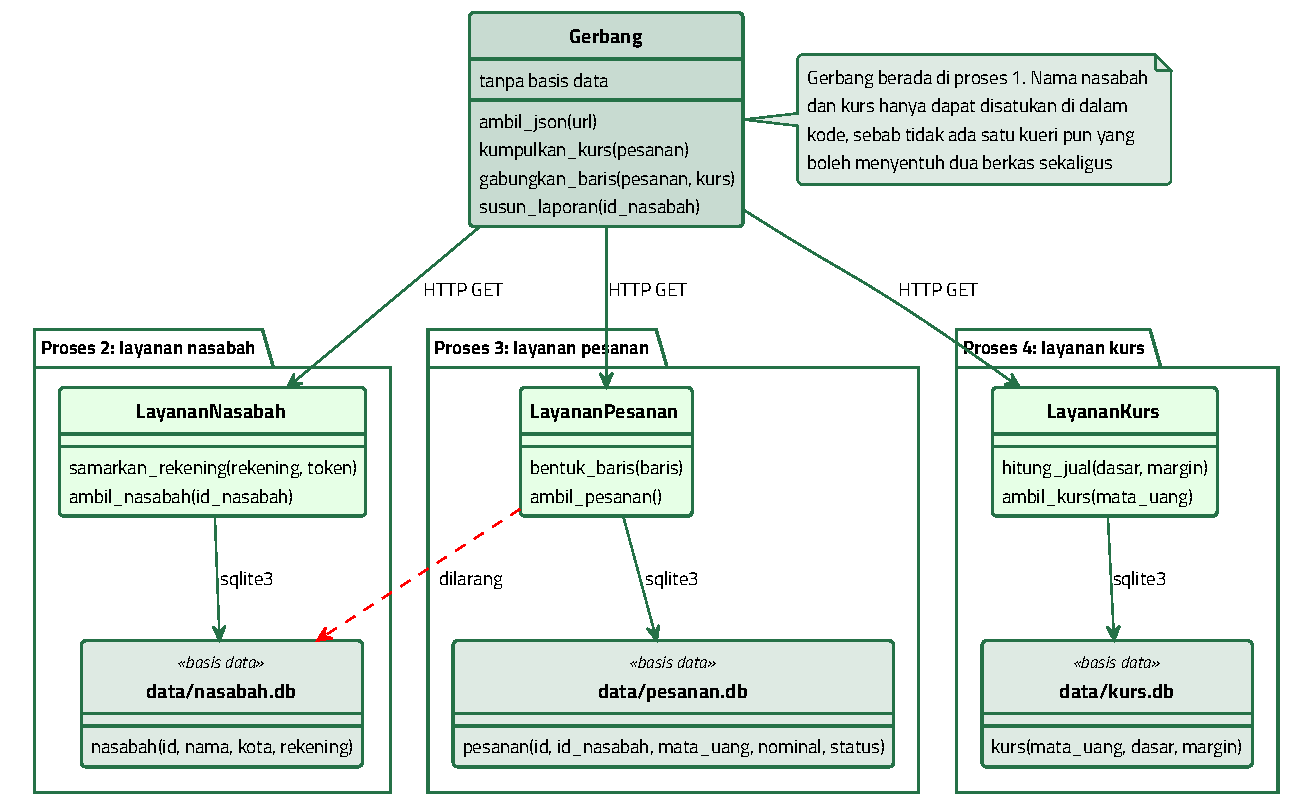
\includegraphics[width=\textwidth, height=0.44\textheight,
    keepaspectratio]{kelas-mikroservis.pdf}
  \caption{Tiga layanan beserta basis datanya masing-masing. Panah merah
    putus-putus adalah jalur yang dilarang, yaitu satu layanan membuka berkas
    milik layanan lain}
  \label{fig:kelas-mikroservis}
\end{figure}

Harga penggabungan itu dapat dihitung, bukan sekadar dirasakan. Skrip
\texttt{ukur\_laporan.py} membaca kode sumbernya sendiri lewat modul
\texttt{ast}, sehingga jumlah barisnya berubah sendiri bila kodenya disunting.
Tabel~\ref{tab:harga-gabung} merangkum ketiga harganya.

\begin{table}[htbp]
  \centering
  \caption{Harga penggabungan satu laporan pada kedua versi, dua ratus putaran}
  \label{tab:harga-gabung}
  \begin{tabularx}{\textwidth}{|X|l|l|}
    \hline
    \textbf{Yang dibandingkan} & \textbf{Monolit} & \textbf{Mikroservis} \\
    \hline
    Median satu laporan & 7,70 ms & 31,65 ms \\
    \hline
    Persentil ke-95 & 24,26 ms & 99,61 ms \\
    \hline
    Terbesar & 38,11 ms & 130,81 ms \\
    \hline
    Baris kode penggabung & 26 & 44 \\
    \hline
    Permintaan jaringan & 1 & 5 \\
    \hline
    Putaran lebih cepat & 200 dari 200 & 0 dari 200 \\
    \hline
  \end{tabularx}
\end{table}

Baris terakhir itulah yang membuat selisihnya layak disebut ada. Menurut ukuran
Bab~2, selisih yang lebih kecil daripada ragam pengukurannya belum dapat
diakui. Di sini pencacahan per putaran menunjuk 200 dari 200, sehingga arahnya
tidak lagi meragukan walaupun angka mutlaknya naik turun mengikuti kesibukan
mesin.

\section{Lompatan Jaringan dan Latensi}

Jumlah permintaan jaringan pada tabel sebelumnya bukan angka taksiran. Setiap
jawaban memuat kunci \texttt{lompatan}, yaitu cacah perjalanan Hypertext
Transfer Protocol (HTTP) yang dibutuhkan satu permintaan, terhitung sejak
permintaan klien. Versi monolit selalu melaporkan satu, sedangkan versi
mikroservis melaporkan angka yang bergantung pada isi pesanannya.

Gambar~\ref{fig:sekuens-mikroservis} memperlihatkan kedua jalur itu
berdampingan. Nasabah N-001 memiliki tiga pesanan lunas dalam dua mata uang,
sehingga gerbang memanggil layanan kurs dua kali.

\begin{figure}[htbp]
  \centering
  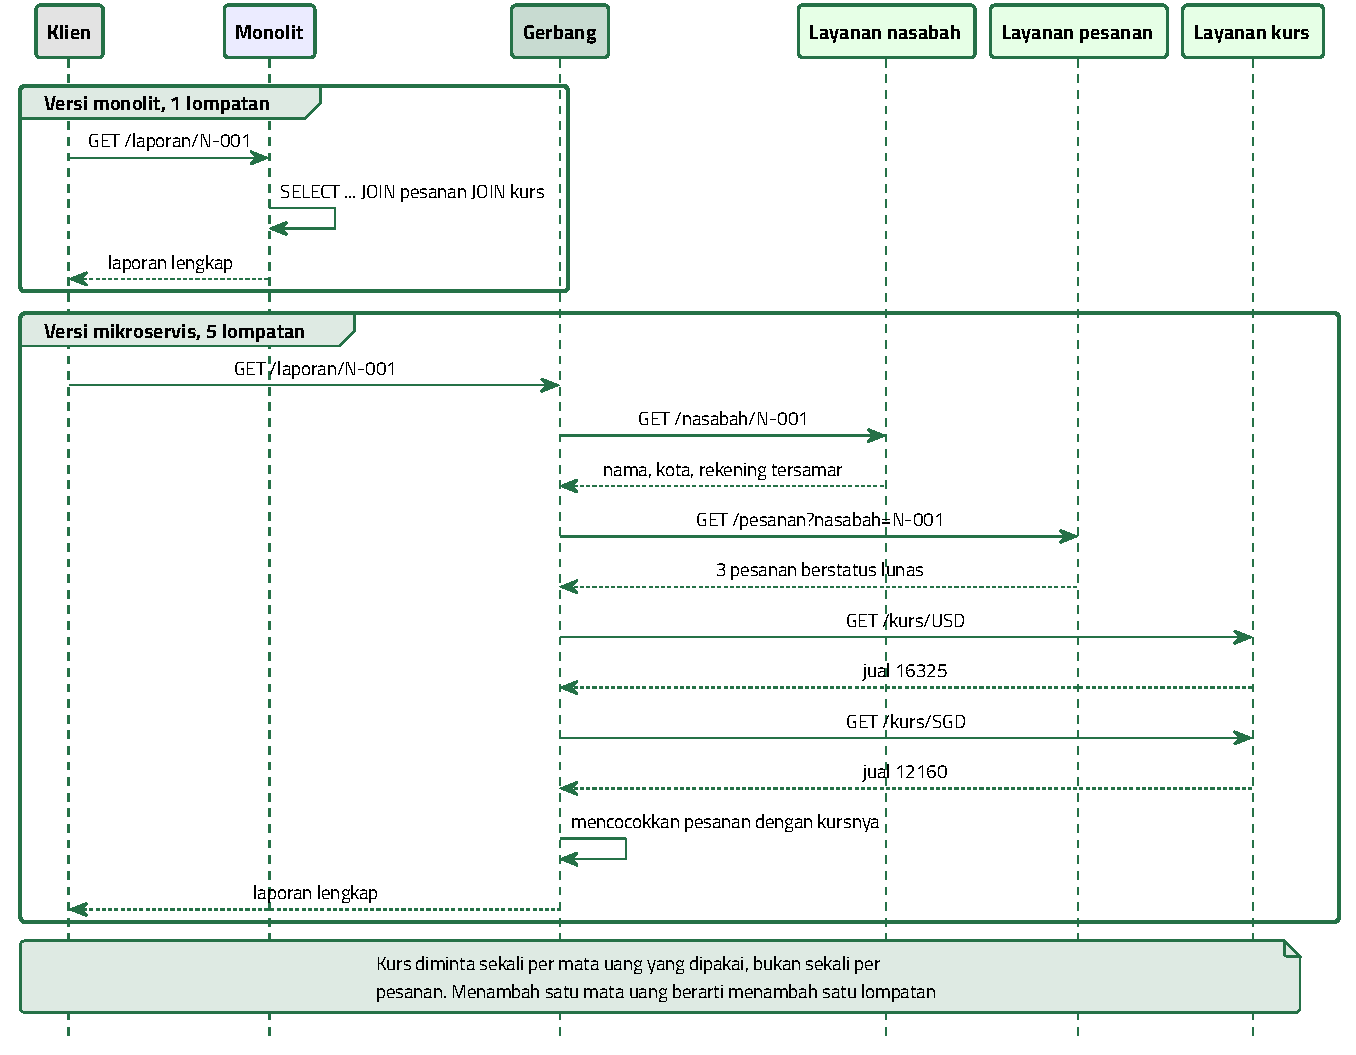
\includegraphics[width=\textwidth, height=0.52\textheight,
    keepaspectratio]{sekuens-mikroservis.pdf}
  \caption{Satu laporan gabungan pada kedua versi. Lompatan tambahannya bukan
    pilihan gaya, melainkan akibat langsung dari basis data yang terpisah}
  \label{fig:sekuens-mikroservis}
\end{figure}

Kurs diminta sekali per mata uang, bukan sekali per pesanan, sebab hasilnya
disimpan sementara di dalam gerbang selama laporan disusun. Penghematan itu
penting, namun tidak mengubah sifat dasarnya. Menambah satu mata uang baru pada
pesanan tetap berarti menambah satu lompatan.

Selisih waktunya diukur dengan menyalakan kedua versi berbarengan pada porta
yang berbeda, lalu mengukur keduanya bergantian di dalam putaran yang sama.
Cara itu dipilih sebab mesin yang sedang sibuk membuat angka mutlaknya naik
turun, sedangkan perbandingan di dalam satu putaran tetap sah.
Tabel~\ref{tab:latensi-lompatan} memuat hasilnya.

\begin{table}[htbp]
  \centering
  \caption{Latensi dan jumlah lompatan dua jenis permintaan, dua ratus putaran}
  \label{tab:latensi-lompatan}
  \begin{tabularx}{\textwidth}{|l|X|l|l|l|l|}
    \hline
    \textbf{Versi} & \textbf{Permintaan} & \textbf{Median} & \textbf{p95} & \textbf{Terbesar} & \textbf{Lompatan} \\
    \hline
    Monolit & nasabah & 12,46 ms & 32,59 ms & 50,33 ms & 1 \\
    \hline
    Monolit & laporan & 12,97 ms & 32,30 ms & 50,81 ms & 1 \\
    \hline
    Mikroservis & nasabah & 17,34 ms & 41,89 ms & 77,04 ms & 2 \\
    \hline
    Mikroservis & laporan & 56,49 ms & 137,82 ms & 202,00 ms & 5 \\
    \hline
  \end{tabularx}
\end{table}

Angka mutlak pada tabel itu perlu dibaca dengan hati-hati. Pengukurannya
dijalankan di mesin yang sedang mengerjakan beberapa pekerjaan lain, sehingga
nilai terbesarnya melonjak sampai empat kali mediannya. Yang tahan terhadap
kesibukan itu adalah perbandingannya. Permintaan nasabah menempuh satu lompatan
tambahan dan menjadi sekitar 1,4 kali lebih lambat, sedangkan permintaan
laporan menempuh empat lompatan tambahan dan menjadi sekitar 4,4 kali lebih
lambat.

Perbandingan itu memberi satu pegangan yang berguna. Biaya mikroservis tumbuh
mengikuti jumlah lompatan, bukan mengikuti jumlah layanan yang terpasang.
Layanan yang banyak tetapi jarang dipanggil bersama tidak mahal, sedangkan tiga
layanan yang selalu dipanggil bersama-sama sudah cukup mahal.

\section{Kegagalan yang Tertahan di Satu Layanan}

Konsekuensi kedua bersifat sebaliknya, yaitu menguntungkan. Pertanyaannya,
apakah matinya satu layanan benar-benar menyisakan layanan lain tetap hidup.

Percobaannya sederhana. Layanan kurs dimatikan, sedangkan layanan nasabah dan
layanan pesanan dibiarkan hidup. Pada versi monolit tidak ada bagian yang dapat
dimatikan sendiri, sehingga yang dimatikan adalah seluruh prosesnya.
Ketimpangan itu bukan kecurangan, melainkan justru inti persoalannya.

Tabel~\ref{tab:kegagalan} memuat hasil percobaan tersebut. Golongan
\textit{sebagian} berarti permintaannya tetap dijawab, namun ada bagian isinya
yang kosong.

\begin{table}[htbp]
  \centering
  \caption{Nasib tiga jenis permintaan ketika kemampuan kurs mati}
  \label{tab:kegagalan}
  \begin{tabularx}{\textwidth}{|l|X|X|}
    \hline
    \textbf{Permintaan} & \textbf{Monolit, proses mati} & \textbf{Mikroservis, layanan kurs mati} \\
    \hline
    nasabah & gagal & penuh \\
    \hline
    kurs & gagal & gagal \\
    \hline
    laporan & gagal & sebagian \\
    \hline
    Terlayani & 0 dari 3 & 2 dari 3 \\
    \hline
  \end{tabularx}
\end{table}

Baris ketiga itu layak diperhatikan. Gerbang sengaja ditulis agar laporannya
tetap keluar ketika layanan kurs bungkam, yaitu dengan nilai rupiah kosong dan
kunci \texttt{lengkap} bernilai \texttt{false}. Nasabah masih dapat melihat
daftar pesanannya, hanya kolom rupiahnya yang hilang. Pilihan itu tidak datang
sendiri, dan ditulis sebagai sembilan baris di dalam gerbang.

Kasus berikut memperlihatkan mengapa pilihan itu dibuat. Sebuah bank memindahkan
sistem penukaran valuta asingnya ke mikroservis. Pada bulan pertama, penyedia
kurs pihak ketiga mengalami gangguan selama empat puluh menit. Layanan kurs ikut
berhenti menjawab, sedangkan layanan nasabah dan layanan pesanan tetap sehat.
Karena gerbangnya menolak menyusun laporan tanpa kurs, seluruh halaman riwayat
menampilkan galat. Petugas cabang tidak dapat melihat daftar pesanan yang sudah
lunas, padahal daftar itu sama sekali tidak membutuhkan kurs. Sesudah gerbangnya
diubah agar menyerahkan laporan tanpa kolom rupiah, gangguan serupa pada bulan
berikutnya hanya menghilangkan satu kolom.

Kemampuan itu tidak gratis. Setiap pemanggilan antar layanan wajib membayangkan
jawaban yang tidak pernah datang, sehingga setiap panggilan butuh tenggang
waktu, penanganan galat, dan keputusan tentang apa yang harus terjadi
sesudahnya. Pada monolit, pemanggilan antar modul tidak pernah menuntut hal
tersebut.

\section{Rilis yang Berdiri Sendiri}

Kurs berubah setiap hari kerja, sehingga layanan kurs adalah bagian yang paling
sering dipasang ulang. Pada versi mikroservis, merilisnya berarti menjalankan
ulang satu proses. Pada versi monolit, kurs tinggal di dalam proses yang sama
dengan nasabah dan pesanan, sehingga merilisnya berarti menjalankan ulang
seluruhnya.

Pengukurannya mengalirkan dua ratus permintaan berjarak tetap dua puluh lima
milidetik, lalu memicu rilis pada permintaan kelima puluh. Jarak tetap itu
membuat jumlah permintaan yang tidak terlayani penuh dapat dibaca langsung
sebagai lama padam. Satu kali rilis tidak cukup, sebab lama nyala sebuah proses
Python bergantung pada kesibukan mesin, sehingga rilisnya diulang tujuh kali
lalu diambil mediannya. Tabel~\ref{tab:rilis} memuat hasilnya.

\begin{table}[htbp]
  \centering
  \caption{Akibat merilis ulang kemampuan kurs, median tujuh kali rilis}
  \label{tab:rilis}
  \begin{tabularx}{\textwidth}{|l|X|l|l|l|}
    \hline
    \textbf{Versi} & \textbf{Lalu lintas} & \textbf{Tidak penuh} & \textbf{Padam} & \textbf{Padam terbesar} \\
    \hline
    Monolit & nasabah & 34 dari 200 & 875 ms & 1.003 ms \\
    \hline
    Monolit & laporan & 35 dari 200 & 846 ms & 981 ms \\
    \hline
    Mikroservis & nasabah & 0 dari 200 & 767 ms & 1.052 ms \\
    \hline
    Mikroservis & laporan & 30 dari 200 & 758 ms & 963 ms \\
    \hline
  \end{tabularx}
\end{table}

Baris ketiga itulah imbalan terbesar mikroservis pada bab ini. Kurs dipasang
ulang, prosesnya benar-benar mati selama lebih dari setengah detik, namun tidak
satu pun permintaan nasabah terganggu. Pada monolit, permintaan nasabah ikut
gagal walaupun nasabah sama sekali tidak berhubungan dengan kurs.

Baris keempat memperlihatkan batasnya. Permintaan laporan memang membutuhkan
kurs, sehingga rilis kurs tetap terasa di situ. Bedanya, terasanya berupa kolom
rupiah yang kosong, bukan berupa halaman galat. Kolom padam pada keempat baris
hampir sama, dan kesamaan itu masuk akal, sebab yang dinyalakan ulang sama-sama
satu proses Python berisi satu aplikasi Flask.

\section{Kapan Pembagian Sehalus Ini Sepadan}

Ketiga pengukuran sebelumnya dapat dibaca sebagai satu neraca. Sisi biayanya
adalah latensi laporan yang menjadi sekitar 4,4 kali dan kode penggabung yang
menjadi 44 baris melawan 26 baris. Sisi imbalannya adalah nol permintaan
nasabah yang gagal selama kurs dirilis, ditambah dua dari tiga permintaan yang
tetap dilayani ketika kurs mati.

Neraca itu bergantung pada satu hal, yaitu seberapa sering data dari beberapa
layanan dibutuhkan bersama-sama. Bila hampir setiap halaman membutuhkan
ketiganya, lompatannya terbayar setiap saat sedangkan kemandirian rilisnya
jarang terpakai. Bila tiap layanan umumnya melayani permintaannya sendiri,
neracanya berbalik.

Kasus berikut memperlihatkan akibat salah membaca neraca itu. Sebuah tim
membangun sistem pembayaran kampus langsung sebagai enam layanan, sebelum
domainnya dipahami dengan baik. Batas antara layanan tagihan dan layanan
pembayaran ternyata ditarik di tempat yang keliru, sebab satu tagihan boleh
dicicil. Memindahkan satu tabel dari layanan tagihan ke layanan pembayaran
menuntut pemindahan data, dua kali rilis, dan satu perubahan kontrak yang harus
disepakati dua tim. Pekerjaan yang pada satu basis kode berupa pemindahan satu
kelas berubah menjadi pekerjaan tiga pekan. Pada akhir semester, empat dari enam
layanan disatukan kembali.

Pengalaman seperti itu yang melatarbelakangi saran Fowler agar sistem baru
dimulai sebagai monolit lebih dahulu. Batas yang benar hampir selalu baru
terlihat sesudah sistemnya dipakai, dan memindahkan batas jauh lebih murah
ketika seluruhnya masih berada di satu basis kode~\cite{fowler2015monolithfirst}.
Tabel~\ref{tab:sepadan} merangkum pegangannya.

\begin{table}[htbp]
  \centering
  \caption{Keadaan yang membuat pembagian sehalus mikroservis sepadan}
  \label{tab:sepadan}
  \begin{tabularx}{\textwidth}{|X|X|}
    \hline
    \textbf{Sepadan ketika} & \textbf{Belum sepadan ketika} \\
    \hline
    Tiap layanan umumnya melayani permintaannya sendiri & Hampir setiap halaman membutuhkan tiga layanan sekaligus \\
    \hline
    Irama perubahan tiap bagian jauh berbeda & Seluruh bagian berubah bersama-sama pada rilis yang sama \\
    \hline
    Batas domainnya sudah terbukti dipakai & Batasnya masih ditebak dan sering berpindah \\
    \hline
    Padamnya satu bagian tidak boleh menjatuhkan bagian lain & Sistemnya memang mati bersama-sama tanpa merugikan siapa pun \\
    \hline
  \end{tabularx}
\end{table}

\section{Ringkasan}

Mikroservis membagi sistem menjadi banyak layanan kecil yang masing-masing
memegang basis datanya sendiri. Aturan itu yang membedakannya dari
\textit{service-based architecture} pada Bab~11, yang layanannya sudah terpisah
namun basis datanya masih satu. Perbedaannya hanya satu baris pada tabel
perbandingan, namun akibatnya terasa di hampir setiap keputusan.

Akibat pertama menyentuh cara menyusun laporan. Tidak ada satu kueri SQL pun
yang boleh menyentuh dua basis data, sehingga klausa \texttt{JOIN} digantikan
kode penggabung di dalam gerbang. Pada contoh bab ini, penggantian itu menaikkan
jumlah permintaan jaringan dari satu menjadi lima, menaikkan baris kode
penggabung dari 26 menjadi 44, dan memperlambat laporannya sekitar 4,4 kali.
Pencacahan per putaran menunjuk 200 dari 200, sehingga arah selisihnya tidak
meragukan.

Akibat kedua menyentuh nasib sistem ketika ada yang mati. Layanan kurs yang
bungkam hanya menghilangkan kolom rupiah, sedangkan monolit yang mati
menghilangkan segalanya. Angkanya dua dari tiga permintaan tetap terlayani
melawan nol dari tiga. Kemampuan itu tidak muncul sendiri, dan gerbangnya harus
ditulis agar sanggup menyerahkan laporan yang tidak lengkap.

Akibat ketiga menyentuh rilis. Merilis kurs pada versi mikroservis tidak
mengganggu satu pun permintaan nasabah, sedangkan merilis kurs pada versi
monolit menggagalkan 34 dari 200 permintaan nasabah. Angka padamnya hampir sama
pada kedua versi, sehingga yang berbeda memang bukan lama padamnya, melainkan
siapa saja yang ikut padam.

Pesan utama bab ini karena itu bukan bahwa layanan harus dibuat sekecil
mungkin, melainkan bahwa batas layanan dan batas data harus ditarik bersamaan.
Menarik keduanya di tempat yang salah lebih mahal daripada tidak menariknya sama
sekali, sebab memperbaikinya menuntut pemindahan data dan kesepakatan lintas
tim. Karena itu banyak sistem sebaiknya dimulai sebagai monolit, lalu dipecah
sesudah batasnya terbukti.

\section{Latihan}

Ketiga latihan berikut memakai satu basis kode yang sama di
\berkas{sources/chapter13/}, tetapi menyasar tiga masalah yang berbeda.
Latihan~1 mengukur latensi beserta jumlah lompatan. Latihan~2 mengukur harga
penggabungan data dari dua basis data terpisah. Latihan~3 mengukur akibat
merilis ulang satu layanan. Hasil setiap mahasiswa dapat berbeda, dan yang
dilaporkan adalah pola perbandingannya, bukan angka mutlaknya.

Penyiapannya dijalankan sekali seperti pada Listing~\ref{lst:venv-ch13}. Bab ini
memakai Flask dan requests, keduanya sudah tercantum pada berkas kebutuhan.
Porta 5300 beserta 5310 sampai 5313 harus kosong sebelum skripnya dijalankan.

\begin{lstlisting}[language=bash, caption={Menyiapkan bahan sebelum ketiga
  latihan, seluruh skrip tersedia di \berkas{sources/chapter13/}},
  label=lst:venv-ch13]
bash sources/siapkan_venv.sh
source .venv/bin/activate
cd sources/chapter13
python basis_data.py
# Keluarannya baris pertama: layanan_nasabah  data/nasabah.db   1 tabel, 3 baris
python penjalan.py mikroservis
# Keluarannya baris pertama: Versi mikroservis menyala, 4 proses.
\end{lstlisting}

Perintah terakhir menyalakan keempat proses sampai dihentikan dengan Ctrl+C.
Seluruh skrip pengukuran menyalakan dan mematikan prosesnya sendiri, sehingga
langkah itu hanya dipakai untuk mencoba jalurnya dengan \texttt{curl}.

\subsection*{Latihan 1: Mengukur Latensi dan Jumlah Lompatan}

Latihan ini membuktikan bahwa biaya mikroservis mengikuti jumlah lompatan, bukan
jumlah layanan yang terpasang. Dua jenis permintaan diukur, yaitu permintaan
yang menyentuh satu sumber data dan permintaan yang menyentuh tiga sumber data.
Langkah kerjanya sebagai berikut.

\begin{enumerate}
  \item Jalankan \texttt{python ukur\_latensi.py}, lalu catat keempat baris
    hasilnya beserta dua baris pencacahan di bawahnya.
  \item Buka \berkas{sources/chapter13/gerbang.py}, lalu temukan baris yang
    menghitung kunci \texttt{lompatan} pada fungsi \texttt{susun\_laporan}.
  \item Panggil \texttt{http://127.0.0.1:5310/laporan/N-002} sesudah menyalakan
    versi mikroservis, lalu catat jumlah lompatannya. Nasabah tersebut hanya
    memiliki satu pesanan dalam satu mata uang.
  \item Jelaskan mengapa jumlah lompatannya berbeda dengan jumlah lompatan
    nasabah N-001.
\end{enumerate}

Tabel~\ref{tab:lat1mikro-contoh} berisi hasil satu kali pengukuran nyata.

\begin{table}[htbp]
  \centering
  \caption{Contoh hasil Latihan 1 yang sudah terisi, dua ratus putaran}
  \label{tab:lat1mikro-contoh}
  \begin{tabularx}{\textwidth}{|l|X|l|l|l|l|}
    \hline
    \textbf{Versi} & \textbf{Permintaan} & \textbf{Median} & \textbf{p95} & \textbf{Terbesar} & \textbf{Lompatan} \\
    \hline
    Monolit & nasabah & 12,46 ms & 32,59 ms & 50,33 ms & 1 \\
    \hline
    Monolit & laporan & 12,97 ms & 32,30 ms & 50,81 ms & 1 \\
    \hline
    Mikroservis & nasabah & 17,34 ms & 41,89 ms & 77,04 ms & 2 \\
    \hline
    Mikroservis & laporan & 56,49 ms & 137,82 ms & 202,00 ms & 5 \\
    \hline
  \end{tabularx}
\end{table}

Nilai terbesar pada tabel itu melonjak sampai empat kali mediannya. Sebabnya
mesin pengukurnya sedang mengerjakan beberapa pekerjaan lain, sehingga sebagian
putaran harus menunggu giliran pemroses. Gejala antrean seperti itu memang hanya
terlihat pada nilai terbesar, dan tidak terlihat pada mediannya.

Isikan hasil pengukuran pada Tabel~\ref{tab:lat1mikro-hasil}.

\begin{table}[htbp]
  \centering
  \caption{Lembar isian Latihan 1}
  \label{tab:lat1mikro-hasil}
  \begin{tabularx}{\textwidth}{|l|X|l|l|l|l|}
    \hline
    \textbf{Versi} & \textbf{Permintaan} & \textbf{Median} & \textbf{p95} & \textbf{Terbesar} & \textbf{Lompatan} \\
    \hline
    Monolit & nasabah & \dots & \dots & \dots & \dots \\
    \hline
    Monolit & laporan & \dots & \dots & \dots & \dots \\
    \hline
    Mikroservis & nasabah & \dots & \dots & \dots & \dots \\
    \hline
    Mikroservis & laporan & \dots & \dots & \dots & \dots \\
    \hline
  \end{tabularx}
\end{table}

Jawab tiga pertanyaan berikut dengan menunjuk angka pada tabel. Pertama,
bandingkan selisih pada permintaan nasabah dengan selisih pada permintaan
laporan, lalu jelaskan mengapa keduanya berbeda jauh. Kedua, hitung biaya
rata-rata satu lompatan dari baris permintaan nasabah, lalu periksa apakah
biaya itu menjelaskan baris permintaan laporan. Ketiga, jelaskan mengapa
pencacahan per putaran lebih dapat dipercaya daripada nilai terbesar ketika
mesinnya sedang sibuk.

\subsection*{Latihan 2: Menghitung Harga Penggabungan}

Latihan ini mengukur harga yang dibayar karena basis datanya terpisah. Laporan
yang sama disusun dua kali, yaitu lewat satu kueri SQL pada monolit dan lewat
tiga panggilan HTTP pada mikroservis. Langkah kerjanya sebagai berikut.

\begin{enumerate}
  \item Jalankan \texttt{python ukur\_laporan.py}, lalu catat kedua belas baris
    laporannya.
  \item Bandingkan \texttt{KUERI\_LAPORAN} pada
    \berkas{sources/chapter13/monolit.py} dengan \texttt{susun\_laporan} pada
    \berkas{sources/chapter13/gerbang.py}. Tunjukkan bagian mana yang
    menggantikan klausa \texttt{JOIN}.
  \item Tambahkan satu pesanan baru bermata uang JPY untuk nasabah N-001 pada
    \texttt{ISI\_AWAL} di \berkas{sources/chapter13/layanan_pesanan.py}, lalu
    tambahkan barisnya pada \texttt{ISI\_AWAL} di
    \berkas{sources/chapter13/layanan_kurs.py}.
  \item Jalankan ulang \texttt{python basis\_data.py} lalu
    \texttt{python ukur\_laporan.py}, kemudian catat perubahan jumlah permintaan
    jaringannya.
\end{enumerate}

Tabel~\ref{tab:lat2mikro-contoh} berisi hasil satu kali pengukuran nyata.

\begin{table}[htbp]
  \centering
  \caption{Contoh hasil Latihan 2 yang sudah terisi, dua ratus putaran}
  \label{tab:lat2mikro-contoh}
  \begin{tabularx}{\textwidth}{|X|l|l|}
    \hline
    \textbf{Yang dilaporkan} & \textbf{Monolit} & \textbf{Mikroservis} \\
    \hline
    Median satu laporan & 7,70 ms & 31,65 ms \\
    \hline
    Persentil ke-95 & 24,26 ms & 99,61 ms \\
    \hline
    Terbesar & 38,11 ms & 130,81 ms \\
    \hline
    Baris kode penggabung & 26 & 44 \\
    \hline
    Permintaan jaringan & 1 & 5 \\
    \hline
    Putaran lebih cepat & 200 dari 200 & 0 dari 200 \\
    \hline
    Isi laporan sama & \multicolumn{2}{l|}{ya} \\
    \hline
  \end{tabularx}
\end{table}

Baris terakhir itu sengaja diperiksa skripnya sendiri. Kedua versi menghasilkan
laporan yang sama persis sesudah kunci \texttt{lompatan} dibuang, sehingga yang
dibandingkan memang harganya, bukan hasilnya.

Isikan hasil pengukuran pada Tabel~\ref{tab:lat2mikro-hasil}.

\begin{table}[htbp]
  \centering
  \caption{Lembar isian Latihan 2}
  \label{tab:lat2mikro-hasil}
  \begin{tabularx}{\textwidth}{|X|l|l|l|}
    \hline
    \textbf{Yang dilaporkan} & \textbf{Monolit} & \textbf{Mikroservis} & \textbf{Sesudah JPY} \\
    \hline
    Median satu laporan & \dots & \dots & \dots \\
    \hline
    Persentil ke-95 & \dots & \dots & \dots \\
    \hline
    Baris kode penggabung & \dots & \dots & \dots \\
    \hline
    Permintaan jaringan & \dots & \dots & \dots \\
    \hline
    Putaran lebih cepat & \dots & \dots & \dots \\
    \hline
  \end{tabularx}
\end{table}

Jawab tiga pertanyaan berikut. Pertama, jelaskan mengapa kueri
\texttt{KUERI\_LAPORAN} tidak dapat ditulis sama sekali pada versi mikroservis,
lalu sebutkan aturan mana yang melarangnya. Kedua, bandingkan kenaikan jumlah
permintaan jaringan sesudah JPY ditambahkan dengan kenaikan pada versi monolit,
lalu jelaskan sebabnya. Ketiga, sebutkan satu cara menurunkan jumlah permintaan
jaringan tanpa menggabungkan kembali basis datanya, lalu sebutkan harga yang
dibayar cara tersebut.

\subsection*{Latihan 3: Merilis Ulang Satu Layanan}

Latihan ini mengukur imbalan terbesar mikroservis, yaitu rilis yang berdiri
sendiri. Layanan kurs dipilih sebab kurs berubah setiap hari kerja, sehingga
bagian itulah yang paling sering dipasang ulang. Langkah kerjanya sebagai
berikut.

\begin{enumerate}
  \item Jalankan \texttt{python uji\_kegagalan.py}, lalu catat ketiga baris
    hasilnya beserta dua baris pencacahan di bawahnya.
  \item Jalankan \texttt{python ukur\_rilis.py}, lalu catat keempat baris
    hasilnya. Skrip tersebut mengulang rilisnya tujuh kali pada tiap baris.
  \item Buka \berkas{sources/chapter13/gerbang.py}, lalu ubah
    \texttt{gabungkan\_baris} sehingga melempar galat ketika kursnya bernilai
    \texttt{None}, bukan menyerahkan nilai kosong.
  \item Jalankan ulang kedua skrip, lalu catat perubahan golongan pada baris
    laporan. Kembalikan kodenya sesudah dicatat.
\end{enumerate}

Tabel~\ref{tab:lat3mikro-contoh} berisi hasil satu kali pengukuran nyata.

\begin{table}[htbp]
  \centering
  \caption{Contoh hasil Latihan 3 yang sudah terisi, median tujuh kali rilis}
  \label{tab:lat3mikro-contoh}
  \begin{tabularx}{\textwidth}{|l|X|l|l|l|}
    \hline
    \textbf{Versi} & \textbf{Lalu lintas} & \textbf{Tidak penuh} & \textbf{Padam} & \textbf{Padam terbesar} \\
    \hline
    Monolit & nasabah & 34 dari 200 & 875 ms & 1.003 ms \\
    \hline
    Monolit & laporan & 35 dari 200 & 846 ms & 981 ms \\
    \hline
    Mikroservis & nasabah & 0 dari 200 & 767 ms & 1.052 ms \\
    \hline
    Mikroservis & laporan & 30 dari 200 & 758 ms & 963 ms \\
    \hline
  \end{tabularx}
\end{table}

Isikan hasil pengukuran pada Tabel~\ref{tab:lat3mikro-hasil}.

\begin{table}[htbp]
  \centering
  \caption{Lembar isian Latihan 3}
  \label{tab:lat3mikro-hasil}
  \begin{tabularx}{\textwidth}{|l|X|l|l|l|}
    \hline
    \textbf{Versi} & \textbf{Lalu lintas} & \textbf{Tidak penuh} & \textbf{Padam} & \textbf{Sesudah diubah} \\
    \hline
    Monolit & nasabah & \dots & \dots & \dots \\
    \hline
    Monolit & laporan & \dots & \dots & \dots \\
    \hline
    Mikroservis & nasabah & \dots & \dots & \dots \\
    \hline
    Mikroservis & laporan & \dots & \dots & \dots \\
    \hline
  \end{tabularx}
\end{table}

Jawab tiga pertanyaan berikut dengan menunjuk angka pada tabel. Pertama,
jelaskan mengapa lalu lintas nasabah pada versi mikroservis sama sekali tidak
terganggu, padahal prosesnya benar-benar ada yang mati. Kedua, jelaskan
perubahan golongan pada baris laporan sesudah langkah ketiga, lalu sebutkan apa
yang sebenarnya hilang bagi pengguna. Ketiga, gabungkan hasil ketiga latihan
menjadi satu keputusan, yaitu tentukan apakah sistem penukaran valuta asing ini
sebaiknya dipecah sehalus ini, lalu sebutkan tiga angka yang menjadi dasar
keputusannya.
